\documentclass{report}
\usepackage[spanish]{babel}
\usepackage{natbib}
\usepackage{url}
\usepackage[utf8]{inputenc}
\usepackage{amsmath}
\usepackage{graphicx}
\graphicspath{{images/}}
\usepackage{parskip}
\usepackage{fancyhdr}
\usepackage{vmargin}
\usepackage{subfig}
\usepackage[hidelinks]{hyperref}
\usepackage{enumerate}
\usepackage[usenames]{color}
\usepackage{soul}
\usepackage{float}
\usepackage[T1]{fontenc}
\usepackage{verbatim}
\usepackage{multicol}
\usepackage{listings}
\usepackage{multirow}
\usepackage{booktabs}
\usepackage{moreverb} 
\usepackage{caption}

\setmarginsrb{2.5 cm}{2.5 cm}{2.5 cm}{2.5 cm}{1 cm}{1.5 cm}{1 cm}{1.5 cm}

\title{\textsc{Identificación de Requerimientos en la Administración de Viáticos}}
\author{Luis Angel Hernández Lázaro\\  Daniel Méndez Cruz. }
\date{\today}

\makeatletter
\let\thetitle\@title
\let\theauthor\@author
\let\thedate\@date
\makeatother

\pagestyle{fancy}
\fancyhf{}
\rhead{\theauthor}
\lhead{\thetitle}
\cfoot{\thepage}
\setcounter{secnumdepth}{5}

\begin{document}

%%%%%%%%%%%%%%%%%%%%%%%%%%%%%%%%%%%%%%%%%%%%%%%%%%%%%%%%%%%%%%%%%%%%%%%%%%%%%%%%%%%%%%%%%

\begin{titlepage}
	\centering
    \vspace*{0.5 cm}
    
    
    \begin{figure}
		\centering
		\subfloat{
			\label{logoCimat}
		    
\includegraphics[scale = 0.15]{images/0cover/logoCimat.png}
		}
	\end{figure}
    \textsc{\LARGE Centro de Investigación en Matemáticas A.C.}\\[1.0 cm]
	\textsc{\Large Maestría en Ingeniería de Software}\\[0.5 cm]
	\textsc{\large Requerimientos de Ingeniería de Software\\Dr. Hugo Arnoldo Mitre Hernández}\\[0.5 cm]
	\rule{\linewidth}{0.2 mm} \\[0.4 cm]
	{ \huge \bfseries \thetitle}\\ \textsc{\large \\ Luis Angel Hernández Lázaro \\ Daniel Méndez Cruz}
	\rule{\linewidth}{0.2 mm} \\[1.5 cm]
	
	\begin{minipage}{0.5\textwidth}
		\begin{flushleft} \large
			\emph{Correo:}\\
			daniel.mendez@cimat.mx
		\end{flushleft}
	\end{minipage}~
	\begin{minipage}{0.4\textwidth}
		\begin{flushright} \large
			\emph{Correo:} \\
			luis.hernandez@cimat.mx
		\end{flushright}
	\end{minipage}\\[2 cm]
		
	{\large \thedate}\\[2 cm]
 
	\vfill
	
\end{titlepage}

%%%%%%%%%%%%%%%%%%%%%%%%%%%%%%%%%%%%%%%%%%%%%%%%%%%%%%%%%%%%%%%%%%%%%%%%%%%%%%%%%%%%%%%%%

\tableofcontents
\pagebreak
\pagebreak

\newpage

%%%%%%%%%%%%%%%%%%%%%%%%%%%%%%%%%%%%%%%%%%%%%%%%%%%%%%%%%%%%%%%%%%%%%%%%%%%%%%%%%%%%%%%%%
\chapter{Identificación del Problema}
    
    \section{Introducción}

    En el problema que se aborda en este trabajo es acerca de las actividades que realizá la L.I.N. \textbf{Jessica Garrido Sánchez}, que es la persona encarga del tramite y la administración correspondientes para las comisiones de realizan investigadores durante la temporada escolar. La L.I.N. \textbf{Jessica} se encarga de gestionar los requisitos y los documentos necesarios para que los investigadores realicen sus comisiones con los recursos necesarios y de esta forma tener el apoyo de la institución educativa, siempre y cuando los investigadores realicen la entrega de sus comprobantes de los gastos al finalizar la comisión.\\\\
Al principio del proceso, los investigadores llenan un cuestionario que sirve para recabar la información básica para generar el oficio de comisión, el cual será validado por la L.I.N. \textbf{Jessica} y a su vez lo envía para su autorización con el Director de CIMAT, en este caso con el Dr. \textbf{Cuauhtémoc Lemus}.\\\\
Previamente se generá una relación de gastos o una solicitud de fondos dependiendo de la opción que el investigador haya seleccionado para su comisión. Una vez realizado este documentos, se procede al envío de la documentación a Guanajuato, los cuales consisten en: Oficio de comisión, relación de gastos e informe de comisión; estos documentos se envían tanto de manera electrónica como física.\\\\
Después de los trámites realizados sólo queda esperar que el departamento de administración ubicado en CIMAT Guanajuato corroboren los documentos y los montos declarados, una vez validados de manera correcta son ellos quienes se encargan de realizar los depósitos a las cuentas bancarias de los investigadores.\\\\
Cabe aclarar que para enviar los documentos a Guanajuato el Dr.\textbf{Cuauhtémoc Lemus} se encarga de firmar los documentos correspondientes a la solicitud de fondos y la relación de gastos, para que del departamento de administración en Guanajuato realice el deposito bancario en tiempo y conforme a la ley orgánica de la institución. 

\chapter{Análisis del Problema}

    En esta sección del trabajo se encuentran descritos los artefactos creados para visualizar el análisis de los requerimientos,entre los artefactos que se han creado se encuentran: \emph{Historias de Usuario}, \emph{Diagrama de Casos de Uso}, \emph{Diagrama de BPMN (Business Process Model and Notacion)} y el \emph{Diagrama de Clases}.\\\\
    Las \emph{Historias de Usuario} son empleadas para describir una funcionalidad que es de gran valor para el usuario del sistema. Son Utilizadas para permitir la comprensión por parte de todo el equipo de desarrollo involucrado, además ayudan a tener una planificación eficaz.\\\\
    Los \emph{Casos de Uso} son empleados para representar la  interacción de cada involucrado en el sistema, el actor puede ser un humano o un sistema, los casos casos de uso son asociados con los actores.\\\\
    El \emph{Diagrama de BPMN} es un estándar para el modelado de procesos de negocios, por medio de una notación para definir desde lo simple hasta lo más complejo. Participan quienes están involucrados en un proceso: personas o organizaciones.\\\\
    El \emph{Diagrama de Clases} muestra las diferentes clases que componen un sistema y cómo se relacionan entre otras. Muestran una clase con sus atributos y métodos, así como sus relaciones, es decir que clases conocen o que clases forman parte de otra clase.
    
    \section{Historias de Usuario}\label{HU}
    A continuación se presentan las Historias de Usuario Identificadas como requerimientos para el usuario. Primero se muestra un listado de las actividades principales identificadas, posteriormente se muestra el detalle de las historias de usuario.
    
    Listado de Actividades Principales:
    \begin{description}
        \item[HU1]: Recabar información de investigadores.
        \item[HU2]: Generar oficio de comisión.
        \item[HU3]: Llenar el cuestionario de datos.
        \item[HU4]: Validar oficio de comisión.
        \item[HU5]: Comprobar fondos del proyecto.
        \item[HU6]: Autorizar los oficios de comisión.
        \item[HU7]: Entregar comprobantes.
        \item[HU8]: Generar relación de Gastos.
        \item[HU9]: Firmar solicitud de fondos.
        \item[HU10]: Firmar el informe de comisión.
    \end{description}
    
    \textbf{Detalle de Historias de Usuario}\\\\
    \fbox{\parbox[b]{\linewidth}{
        \begin{description}
            \item[<<Etiqueta>>]: HU1
            \begin{description}
                \item[``Yo como]: Asistente.
                \item[quiero]: Obtener información especifica de los Investigadores.
                \item[para]: Poder generar el oficio de comisión''.
            \end{description}
            \item[<<Fecha>>]: 8-Dic-15
            \item[<<Responsable>>]: Jessica Garrido Sánchez
        \end{description}
    }}
    
    \fbox{\parbox[b]{\linewidth}{
        \begin{description}
            \item[<<Etiqueta>>]: HU2
            \begin{description}
                \item[``Yo como]: Asistente.
                \item[quiero]: Generar oficio de comisión.
                \item[para]: Reembolsar gastos de los Investigadores''.
            \end{description}
            \item[<<Fecha>>]: 8-Dic-15
            \item[<<Responsable>>]: Jessica Garrido Sánchez
        \end{description}
    }}
    
    \fbox{\parbox[b]{\linewidth}{
        \begin{description}
            \item[<<Etiqueta>>]: HU3
            \begin{description}
                \item[``Yo como]: Investigador.
                \item[quiero]: Llenar el cuestionario de datos.
                \item[para]: Obtener el oficio de comisión''.
            \end{description}
            \item[<<Fecha>>]: 8-Dic-15
            \item[<<Responsable>>]: Investigador (es)
        \end{description}
    }}
    
    \fbox{\parbox[b]{\linewidth}{
        \begin{description}
            \item[<<Etiqueta>>]: HU4
            \begin{description}
                \item[``Yo como]: Asistente.
                \item[quiero]: Validar oficio de comisión.
                \item[para]: Evitar problemas en el proceso de reembolso de gastos.''.
            \end{description}
            \item[<<Fecha>>]: 8-Dic-15
            \item[<<Responsable>>]: Jessica Garrido Sánchez
        \end{description}
    }}

    \fbox{\parbox[b]{\linewidth}{
        \begin{description}
            \item[<<Etiqueta>>]: HU5
            \begin{description}
                \item[``Yo como]: Director
                \item[quiero]: Comprobar fondos del Proyecto
                \item[para]: Aprobar las solicitudes de comisión''.
            \end{description}
            \item[<<Fecha>>]: 8-Dic-15
            \item[<<Responsable>>]: Dr.Cuauhtémoc Lemus
        \end{description}
    }}
    
    
    \fbox{\parbox[b]{\linewidth}{
        \begin{description}
            \item[<<Etiqueta>>]: HU6
            \begin{description}
                \item[``Yo como]: Director.
                \item[quiero]: Autorizar los oficios de comisión.
                \item[para]:  Conceder la comisión al investigador''.
            \end{description}
            \item[<<Fecha>>]: 8-Dic-15
            \item[<<Responsable>>]: Dr. Cuauhtémoc Lemus
        \end{description}
    }}
    
    \fbox{\parbox[b]{\linewidth}{
        \begin{description}
            \item[<<Etiqueta>>]: HU7
            \begin{description}
                \item[``Yo como]: Investigador.
                \item[quiero]: Entregar comprobantes .
                \item[para]: Devolver dinero que se gastó en la comisión''.
            \end{description}
            \item[<<Fecha>>]: 8-Dic-15
            \item[<<Responsable>>]: Investigadores
        \end{description}
    }}    
    
    \fbox{\parbox[b]{\linewidth}{
        \begin{description}
            \item[<<Etiqueta>>]: HU8
            \begin{description}
                \item[``Yo como]: Asistente.
                \item[quiero]: Generar relación de gastos / solicitud de fondos.
                \item[para]: Enviar a firma con el Director''.
            \end{description}
            \item[<<Fecha>>]: 8-Dic-15
            \item[<<Responsable>>]: Jessica Garrido Sánchez
        \end{description}
    }}

    \fbox{\parbox[b]{\linewidth}{
        \begin{description}
            \item[<<Etiqueta>>]: HU9
            \begin{description}
                \item[``Yo como]: Director.
                \item[quiero]: Firmar relación de gastos / solicitud de fondos. 
                \item[para]: Enviar documentos a Guanajuato''.
            \end{description}
            \item[<<Fecha>>]: 8-Dic-15
            \item[<<Responsable>>]: Dr.Cuauhtémoc Lemus
        \end{description}
    }}
    
    \fbox{\parbox[b]{\linewidth}{
        \begin{description}
            \item[<<Etiqueta>>]: HU10
            \begin{description}
                \item[``Yo como]: Investigador.
                \item[quiero]: Firmar el informe de comisión
                \item[para]: Solicitar el reembolso de los gastos por la comisión''.
            \end{description}
            \item[<<Fecha>>]: 8-Dic-15
            \item[<<Responsable>>]: Investigador (es)
        \end{description}
    }}
    
       
    \section{Diagrama de Casos de Uso}
    
    En esta sección se muestra el diagrama de casos de uso, propuesto para el análisis de requerimientos (Figura \ref{useCase}), conformado por 16 Casos de Uso. A continuación se muestra una breve descripción  de los casos de uso identificados.\\
    \begin{enumerate}
        \item Asistente    
        \begin{description}
            \item[Enviar Documentación]: Caso de Uso para enviar el expediente de comisión a Guanajuato.
            \begin{description}
                \item[Documentación Electrónica]: Caso de Uso para enviar el expediente de manera electrónica a las oficinas en Guanajuato.
                \item[Documentación Física]: Caso de Uso para enviar el expediente de manera física a las oficinas en Guanajuato.
            \end{description}
            \item[Validar Comprobantes de Viáticos]: Caso de Uso para verificar que los comprobantes tengan la información correcta.
            \item[Registrar Comprobantes]: Caso de uso para registrar comprobantes de la comisión realizada por el investigador
            \item[Generar Oficio de Comisión]: Caso de uso para imprimir el oficio de comisión del investigador.
            \begin{description}
                \item[Validar Oficio de Comisión]: Caso de uso para comprobar la información del oficio de comisión.
            \end{description}
            \item[Generar Informe de Comisión]: Caso de uso para imprimir el informe de comisión del investigador. 
            \begin{description}
                \item[Validar Informe de Comisión]: Caso de uso para comprobar la información del informe de comisión.
            \end{description}
            \item[Generar Relación de Gastos]: Caso de uso para generar la relación de gastos de los viáticos originados  durante la comisión.
            \begin{description}
                \item[Registrar Viáticos Alimentos]: Caso de uso para generar la relación de gastos de tipo Alimentos.
                \item[Registrar Viáticos Hospedaje]: Caso de uso para generar la relación de gastos de tipo Hospedaje.
                \item[Registrar Viáticos Transporte]: Caso de uso para generar la relación de gastos de tipo Transporte.
            \end{description}
        \end{description}    
        \item Docente
        \begin{description}
            \item[LLenar Encuesta de Comisión]: Caso de uso para registrar la información necesaria para generar el oficio de comisión y el informe de comisión.
        \end{description}
        \item Director
        \begin{description}
            \item[Verificar Fondos]: Caso de Uso para comprobar si el proyecto tiene fondos para autorizar la comisión.
            \item[Autorizar Oficio de Comisión]: Caso de uso para autorizar la comisión al investigador.
                \begin{description}
                    \item[Validar Oficio de Comisión]: Caso de uso para validar la información del oficio de comisión. 
                \end{description}
        \end{description}
    \end{enumerate} 

    \begin{figure}[H]
		\begin{center}
		    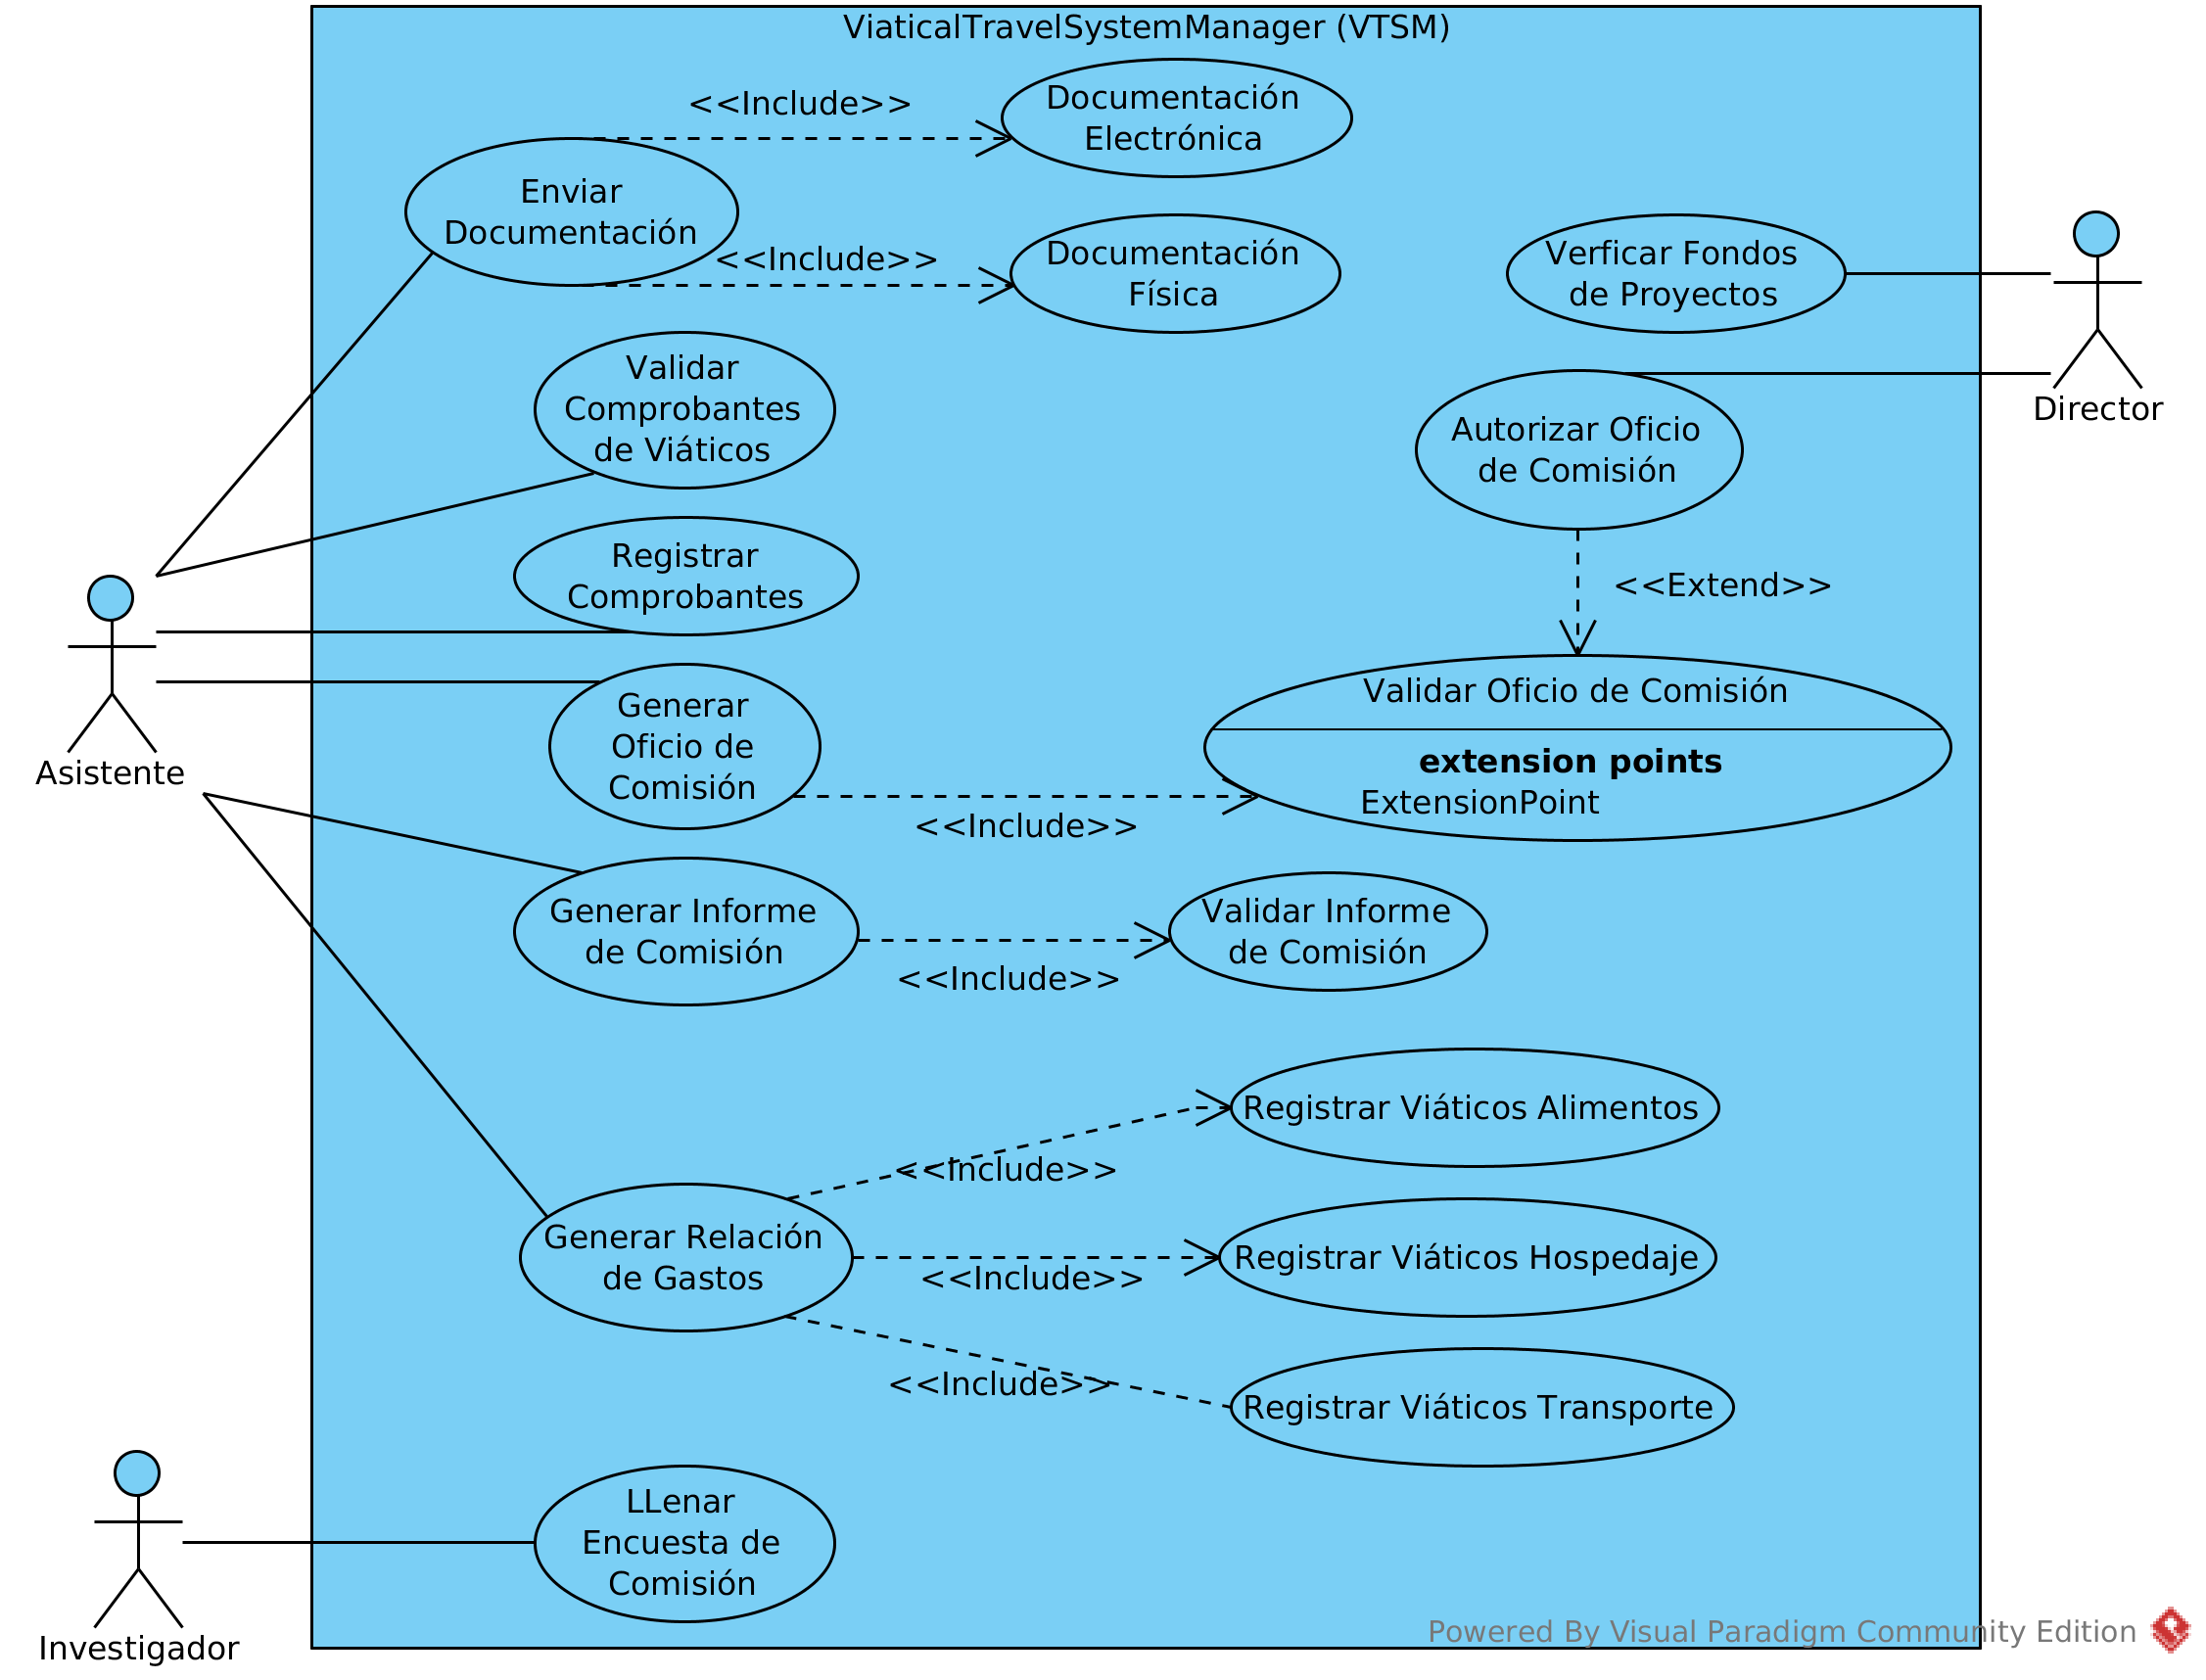
\includegraphics[scale = 0.80]{images/1models/useCase.png}
			\caption{Diagrama de Casos de Uso} 
		\end{center}
        \label{useCase}	
	\end{figure}    
    
    \section{Diagrama BPMN (Business Process Model and Notacion)}
    En esta sección se muestra el diagrama de Business Process Model and Notation (Figura \ref{BPMN}), el cual describe el proceso para administrar las comisiones realizadas por los Investigadores.
    A continuación se presenta el flujo normal para realizar el proceso:
    \begin{enumerate}
        \item fondos
        \item autorización
    \end{enumerate}
    	\begin{figure}
    		\begin{center}
    			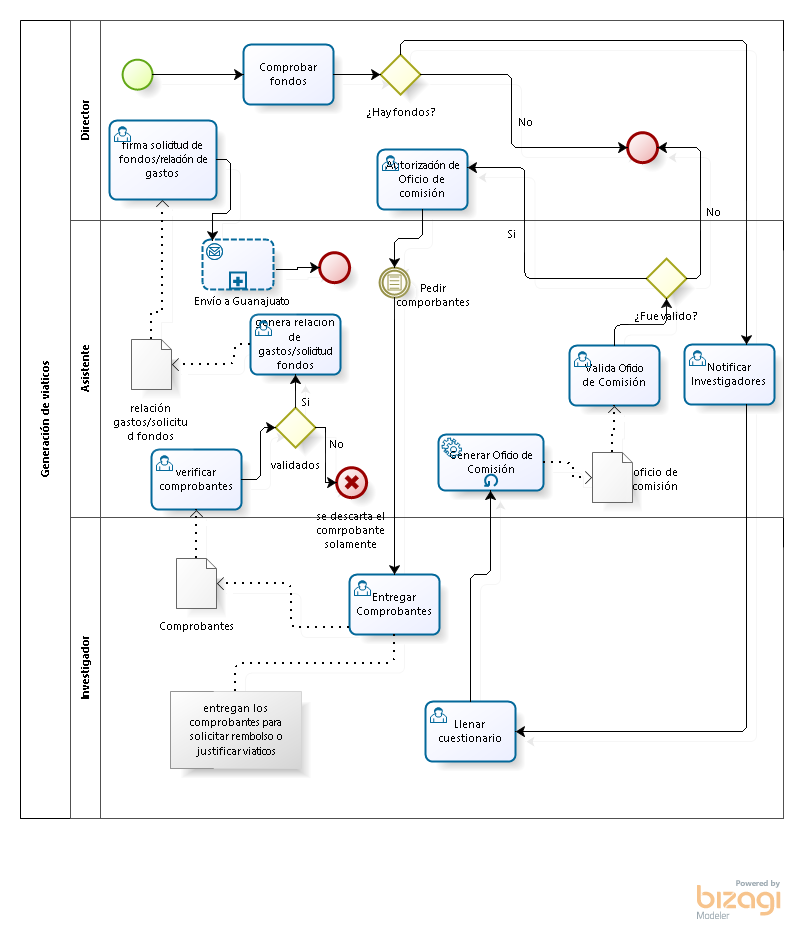
\includegraphics[scale=0.70]{images/1models/comision.png}  
    			\caption{Diagrama BPMN}  		
    		\end{center}
            \label{BPMN}
    	\end{figure}
    En la Figura \ref{subProcesoBPMN} se muestra el subproceso para realizar el reembolso desde el departamento administrativo en CIMAT Guanajuato.

    	\begin{figure}[H]
    		\begin{center}
    			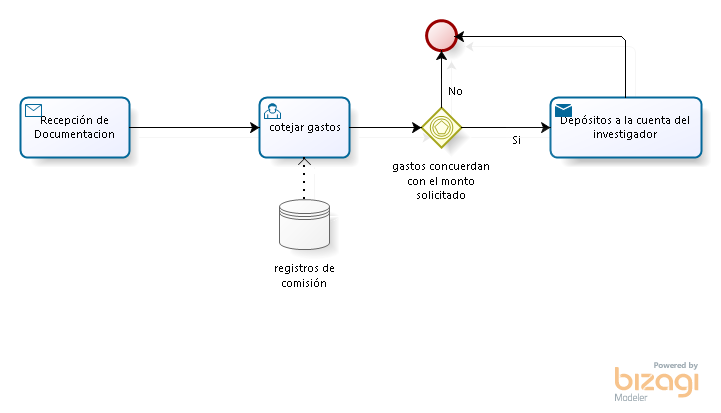
\includegraphics[scale=0.80]{images/1models/envioGto.png}
    			\caption{Diagrama BPMN Subproceso}
    		\end{center}
            \label{subProcesoBPMN}
    	\end{figure}
    
    \section{Diagrama de clases}
    En esta sección se muestra el diagrama de clases (Figura \ref{classDiagram}) identificado con base en las historias de usuario y nuestros casos de uso (Sección \ref{HU}).
      	\begin{figure}
            \begin{center}
    			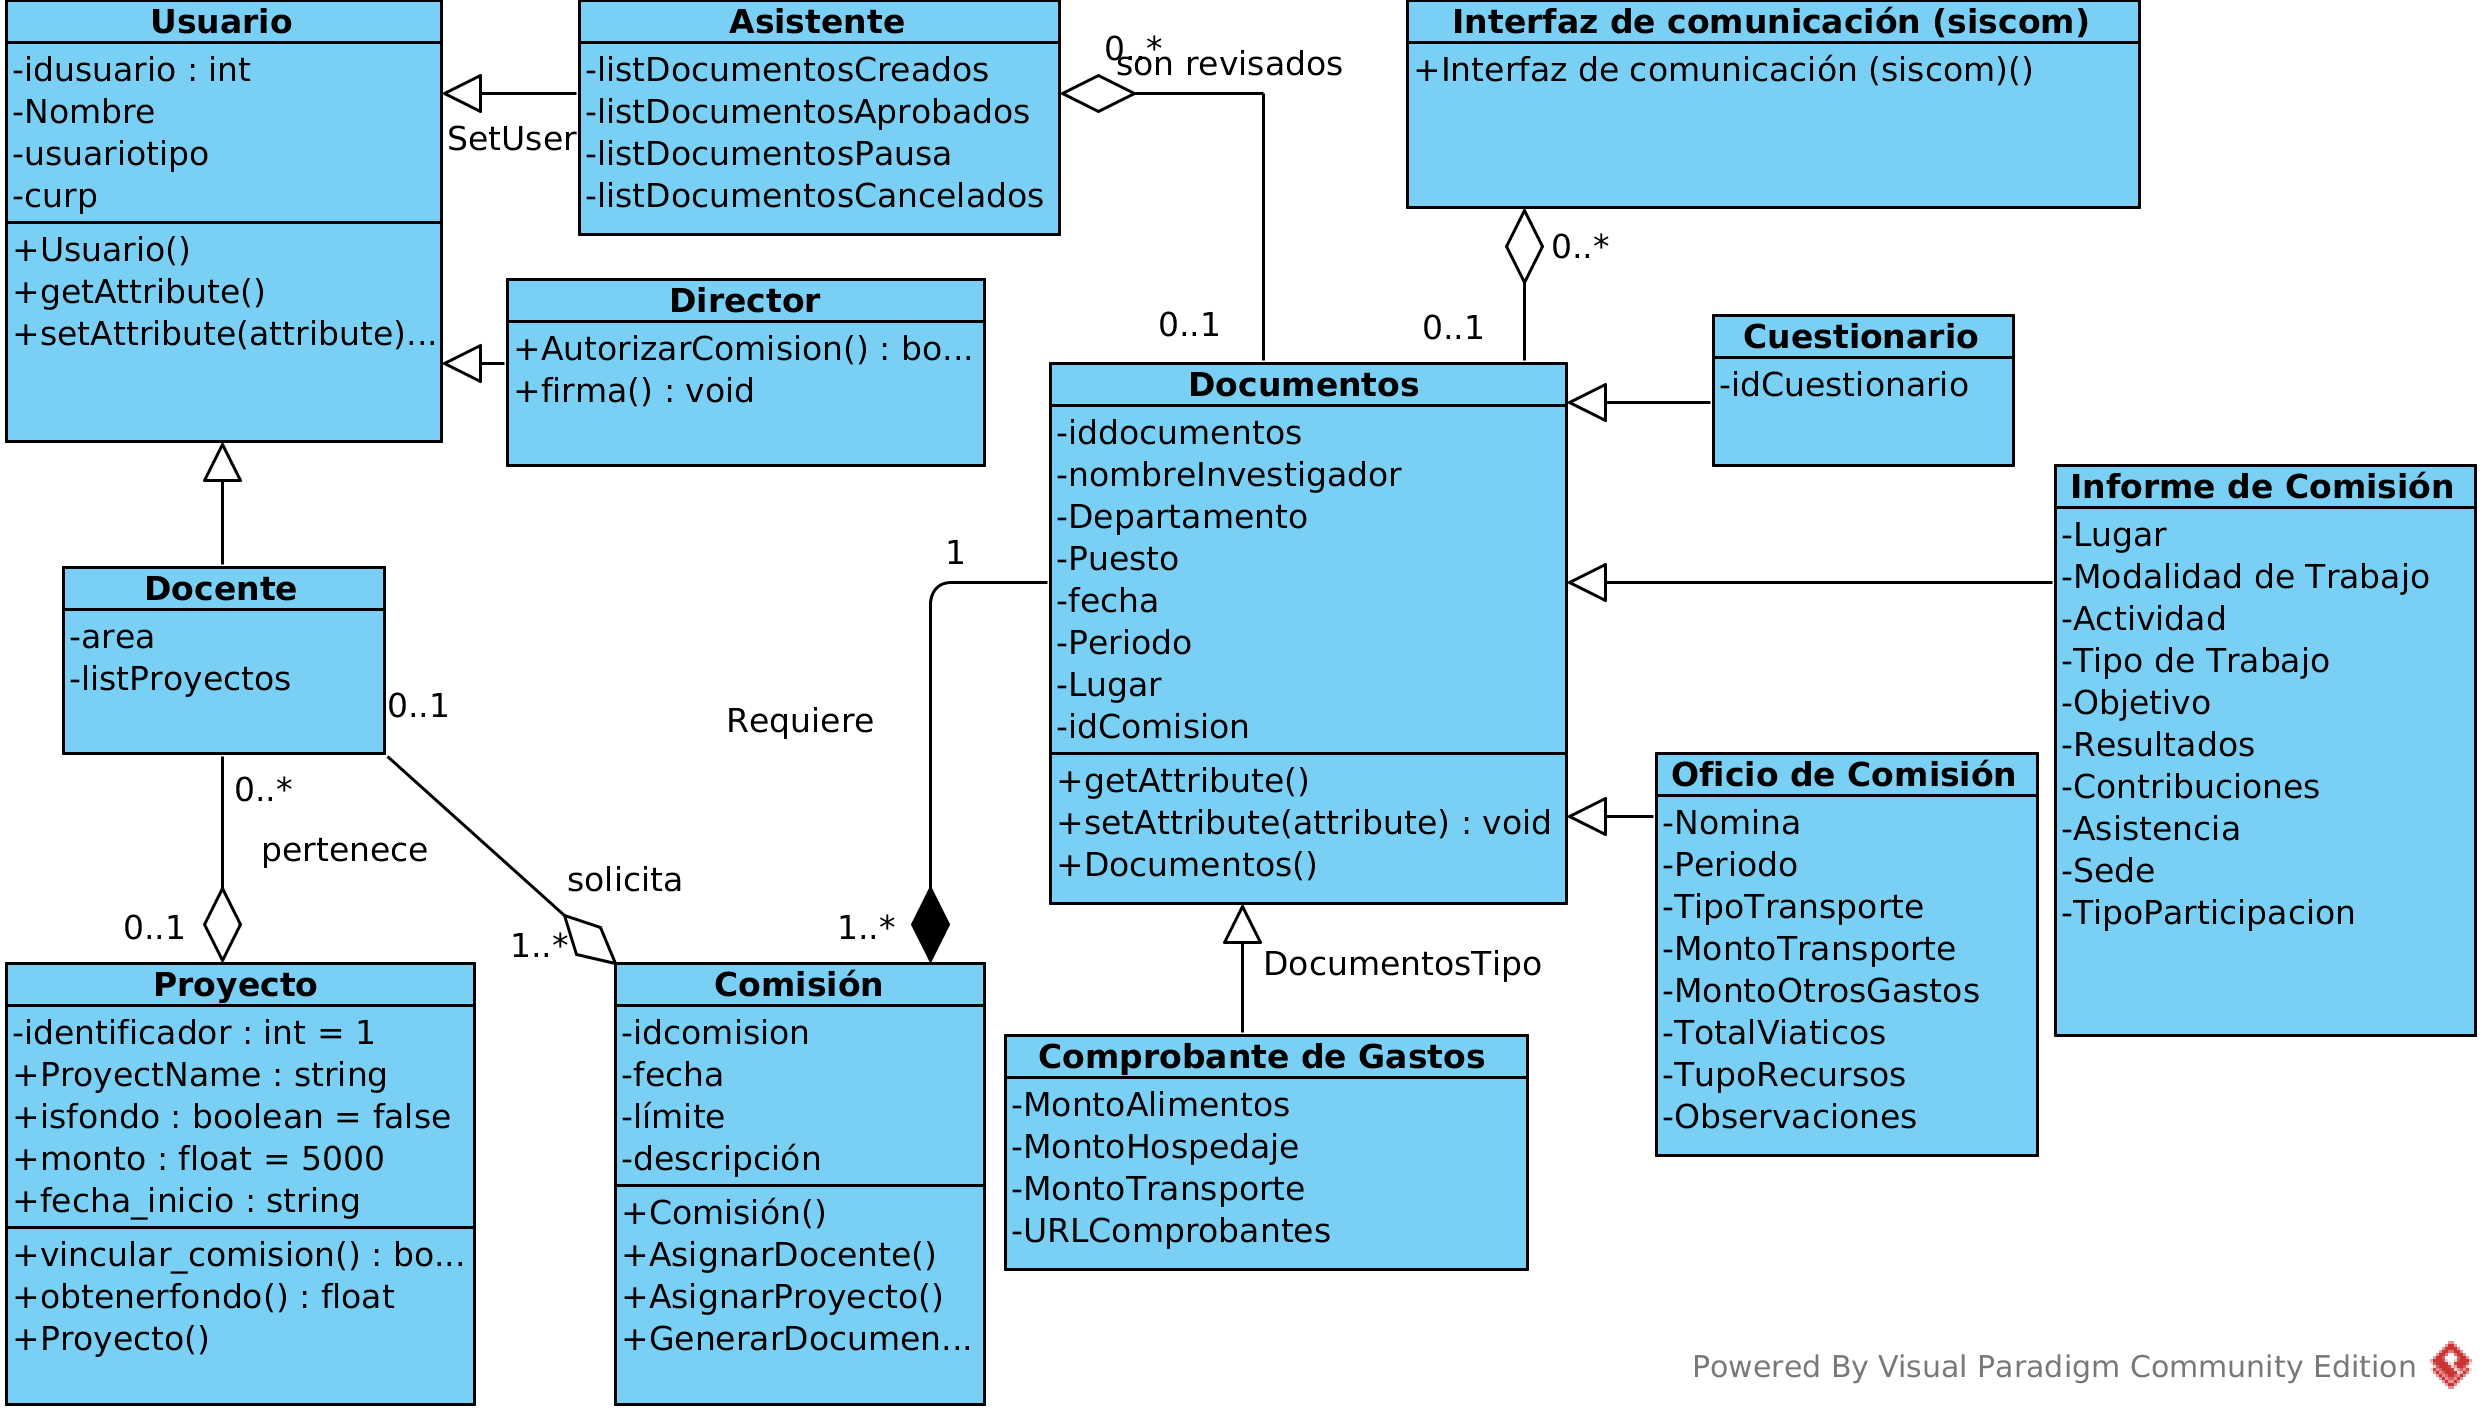
\includegraphics[scale=0.80]{images/1models/DiagramaClases.png}
    			\caption{Diagrama de Clases}
    	    \end{center}
            \label{classDiagram}
    	\end{figure}
       
\chapter{Lecciones Aprendidas}
    
    \section{conclusiones}
    Como resultado del análisis de requerimientos acerca del proceso para administrar los viáticos en las comisiones de los investigadores, es posible concluir que existe una gran importancia en la elicitación de requerimientos, debido a la comunicación con los clientes, los usuarios del sistema y otras personas que tengan relación sobre el producto de software a desarrollar.\\\\
Además el uso de Historias de Usuario reduce el tiempo para la identificación de casos de uso, describiendo las actividades en forma directa y eliminando la ambigüedad que pueda originarse. Las historias de usuario permitieron identificar a los actores y las actividades a desarrollar, comprobando las necesidades básicas para llevar a cabo la administración de viáticos al finalizar las comisiones de los investigadores.
    
    \section{Trabajos Futuros}
    Como trabajo futuro, proponemos realizar la eliminación de la ambigüedad en el proceso para llevar a cabo la administración de los viáticos, debido a que el proceso debe quedar aclarado para realizar un aporte de mejora al proceso en cuestión de automatización, además esto permitirá reforzar los conocimientos adquiridos durante la materia de \emph{Ingeniería de Requerimientos} impartida por el Dr. Hugo Arnoldo Mitre Hernández, en el ciclo escolar: Agosto 2015 - Enero 2016.

\end{document}
